This chapter elaborates on how the model was trained and compared with other techniques from classical computer vision. 

\section{Exploratory analysis}

Drone images from three different towns in the state of Oaxaca where obtained from the National Center for Disaster Prevention (CENAPRED). This pictures where taken during the week following an earthquake that originated in the Pacific coast of the state. We have 727 images from Santa Maria Xadani, 1872 from Union Hidalgo, and 1134 images from Juchitan of Zaragoza. As we can see in the following figures, the drones fly in a regular pattern forming a lattice of points where the images are taken. It is natural to think that given the spatial distribution, that the images are spatialy clustered. We wanted to show that this clustering translates to the space of the information that the images contain. In order to do this, a usual technique was applied to our set of images.

\begin{figure}[h]
  \begin{center}
    \subfigure{\label{fig:tsne}\fbox{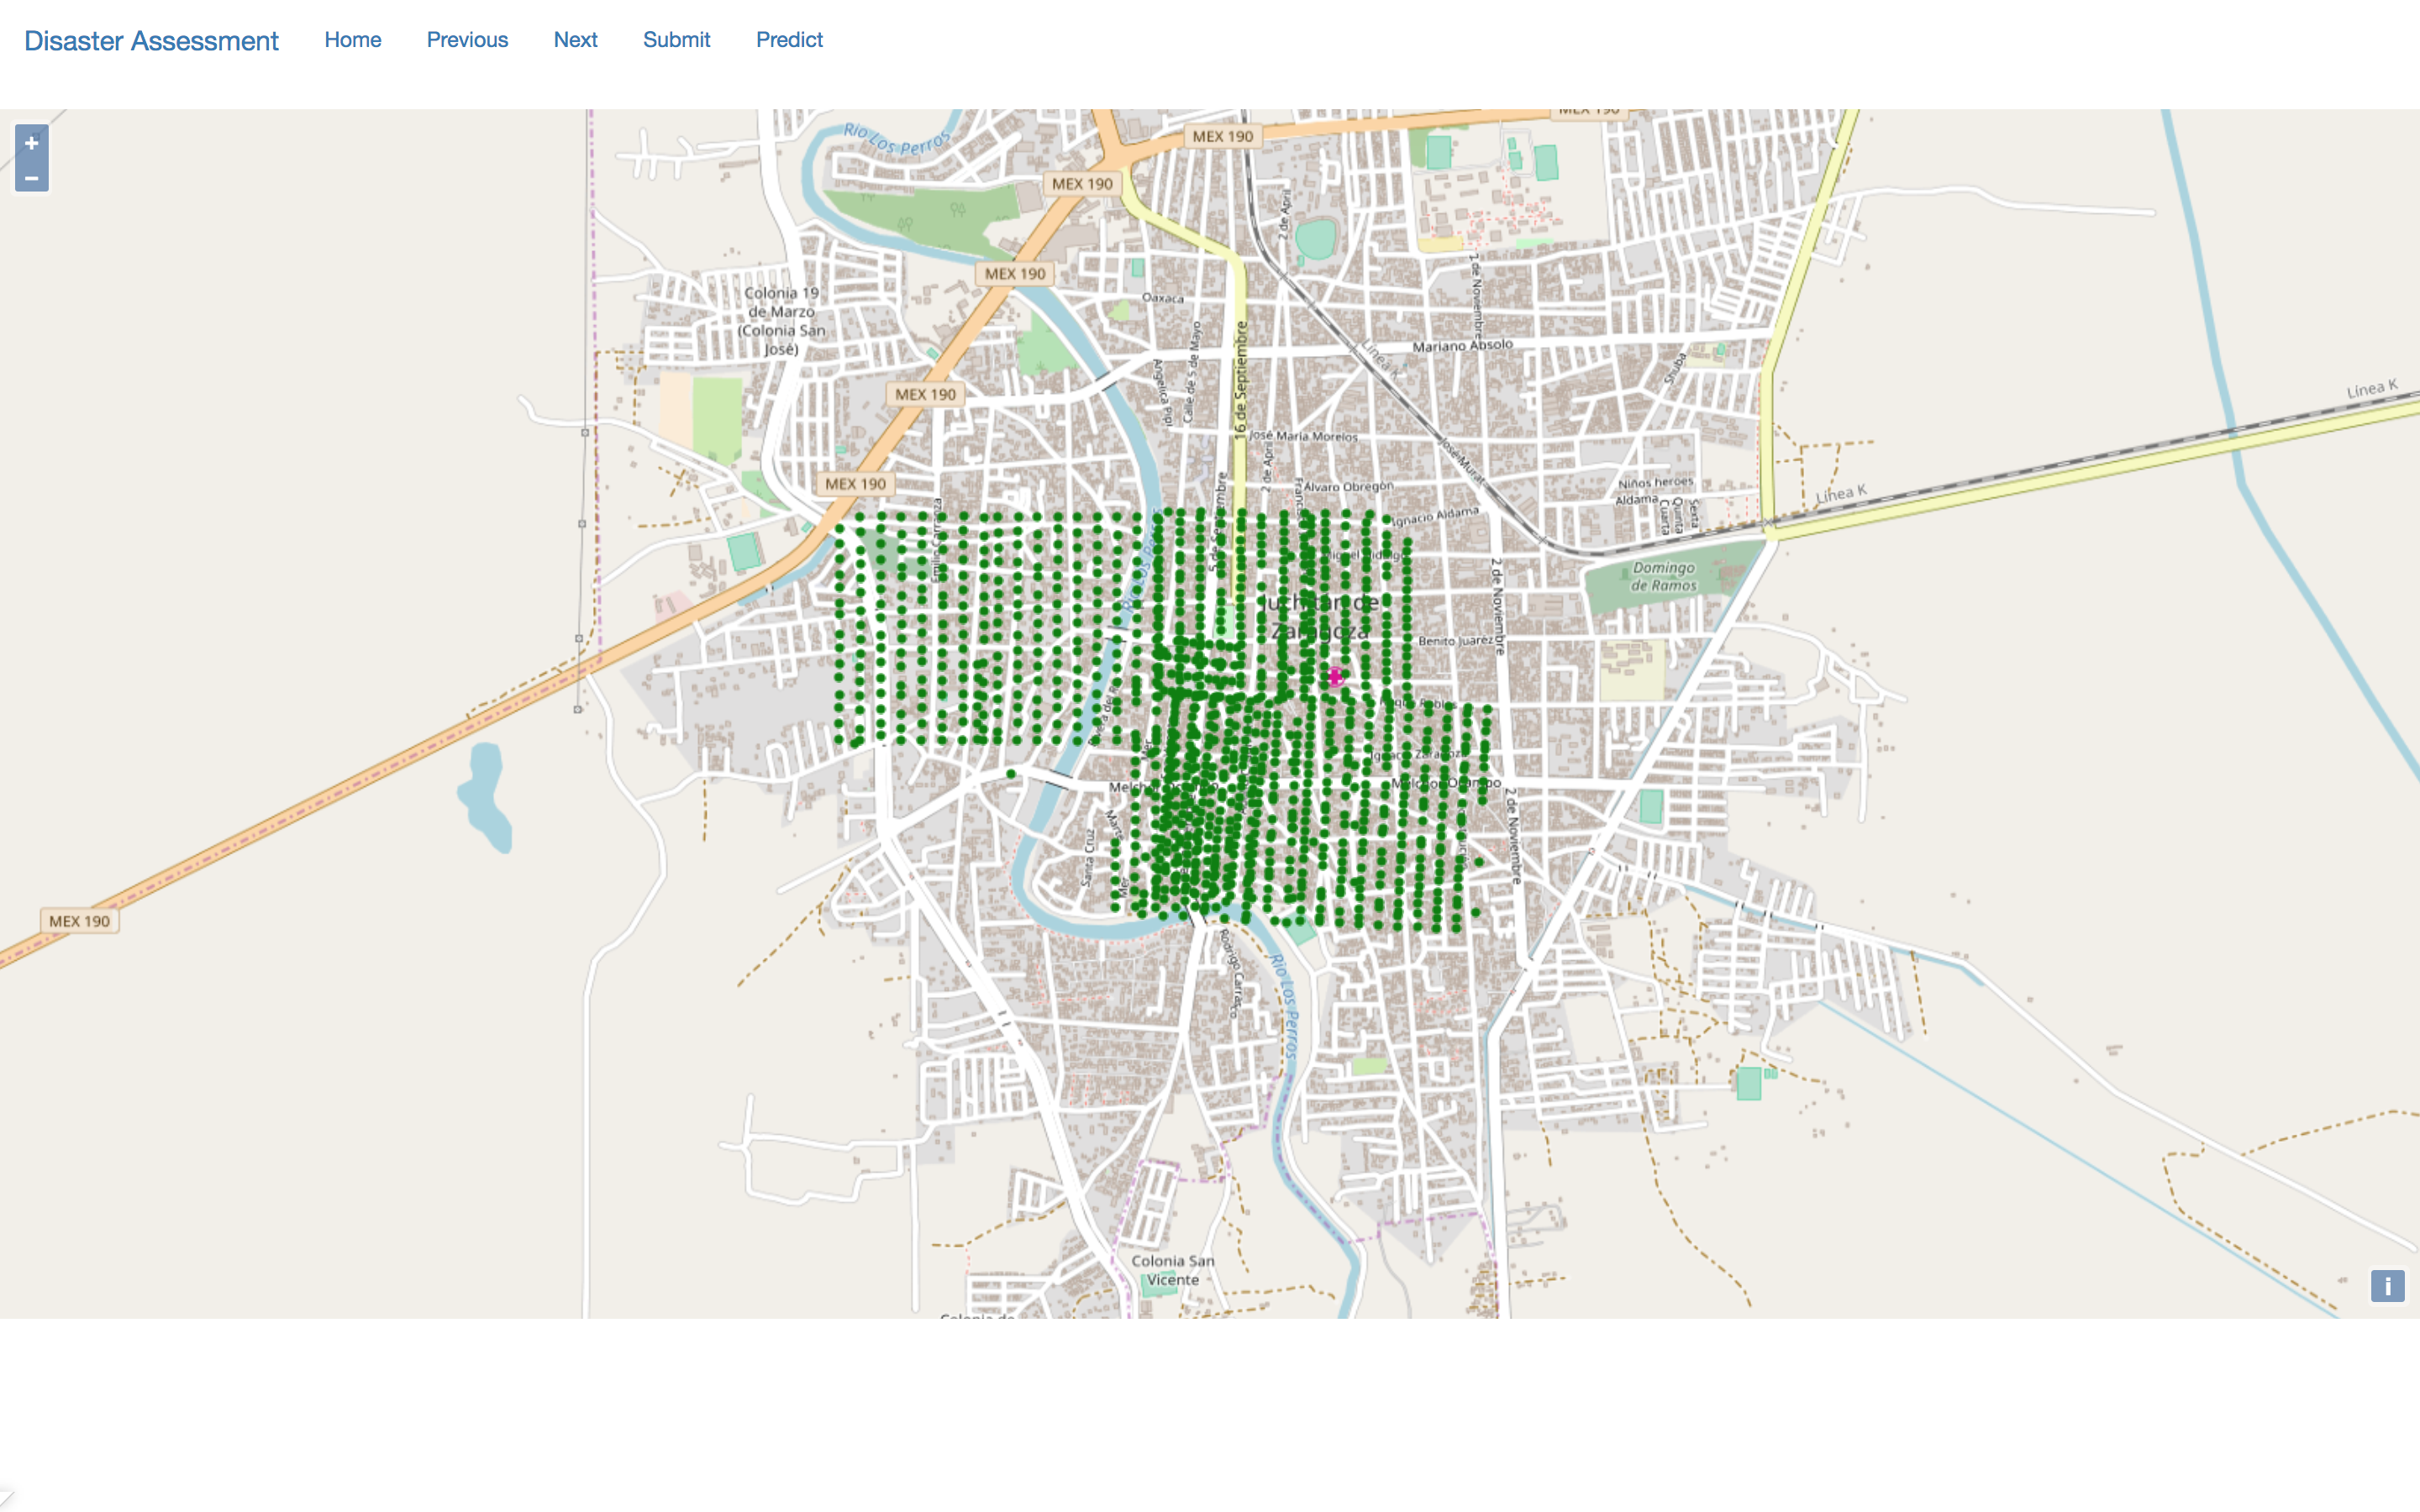
\includegraphics[width=1\textwidth]{images/juchitan.png}}}
  \end{center}
\end{figure}

\begin{figure}[h]
  \begin{center}
    \subfigure{\label{fig:tsne}\fbox{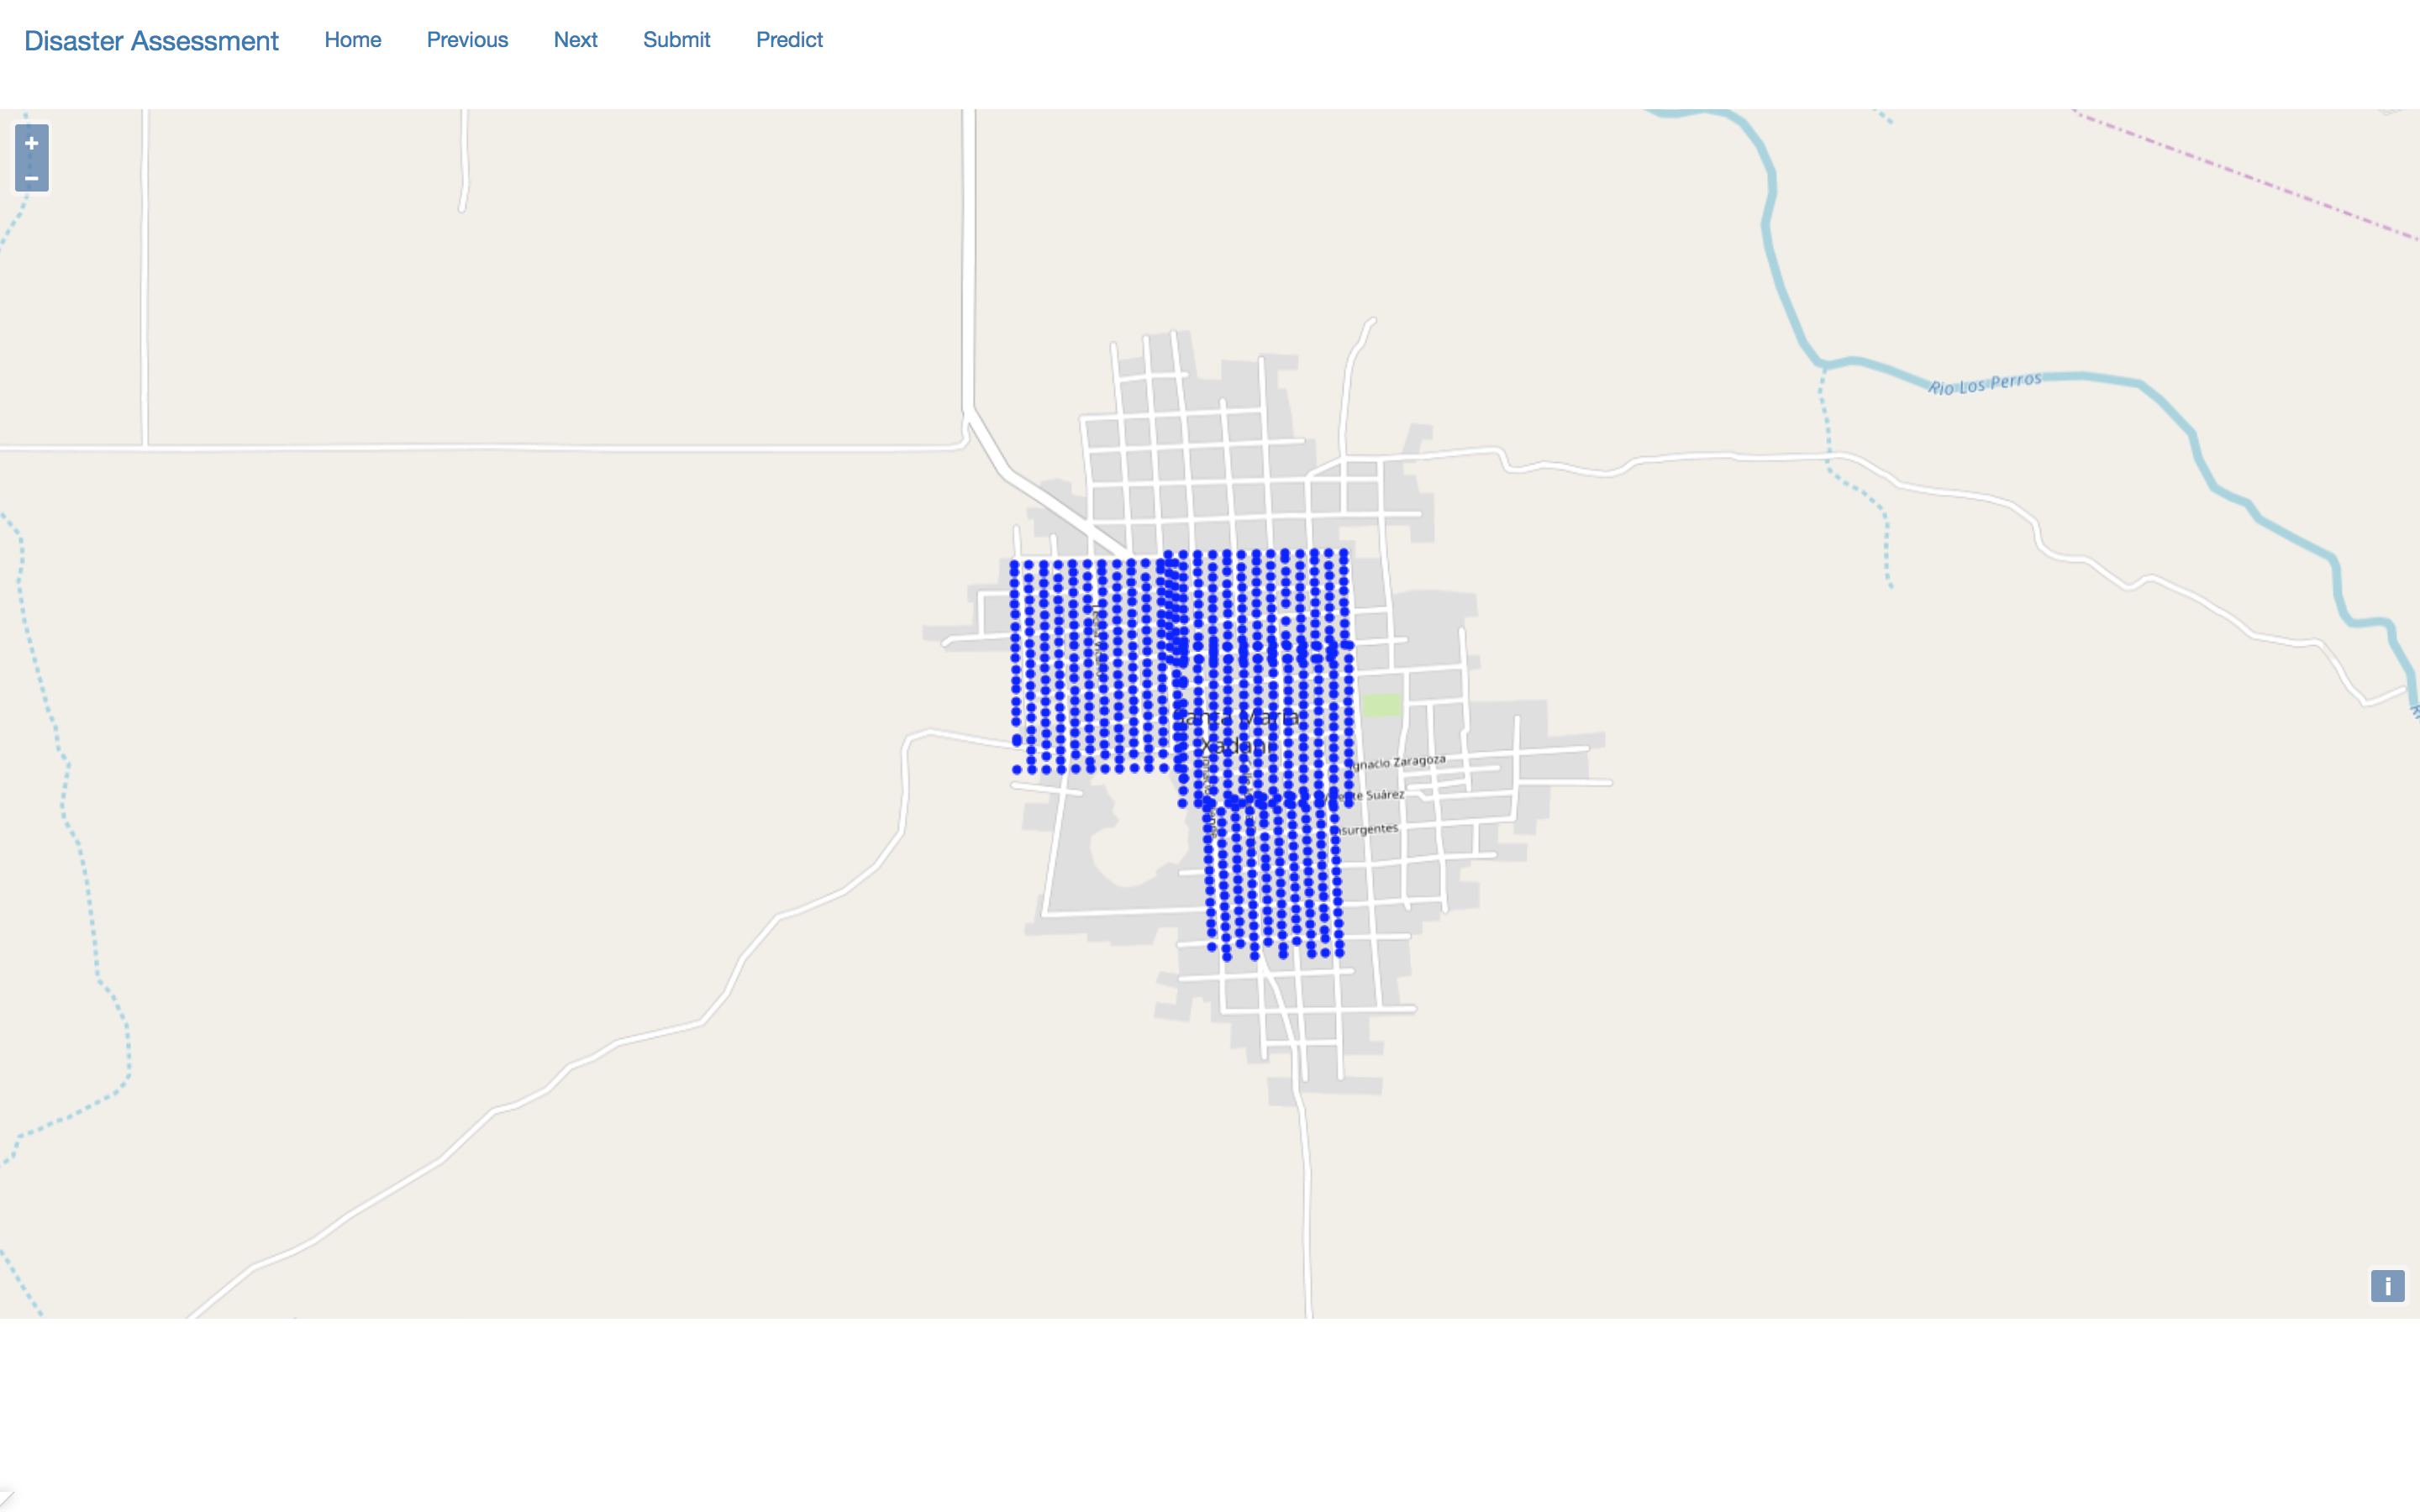
\includegraphics[width=1\textwidth]{images/xadani.png}}}
  \end{center}
\end{figure}

\begin{figure}[h]
  \begin{center}
    \subfigure{\label{fig:tsne}\fbox{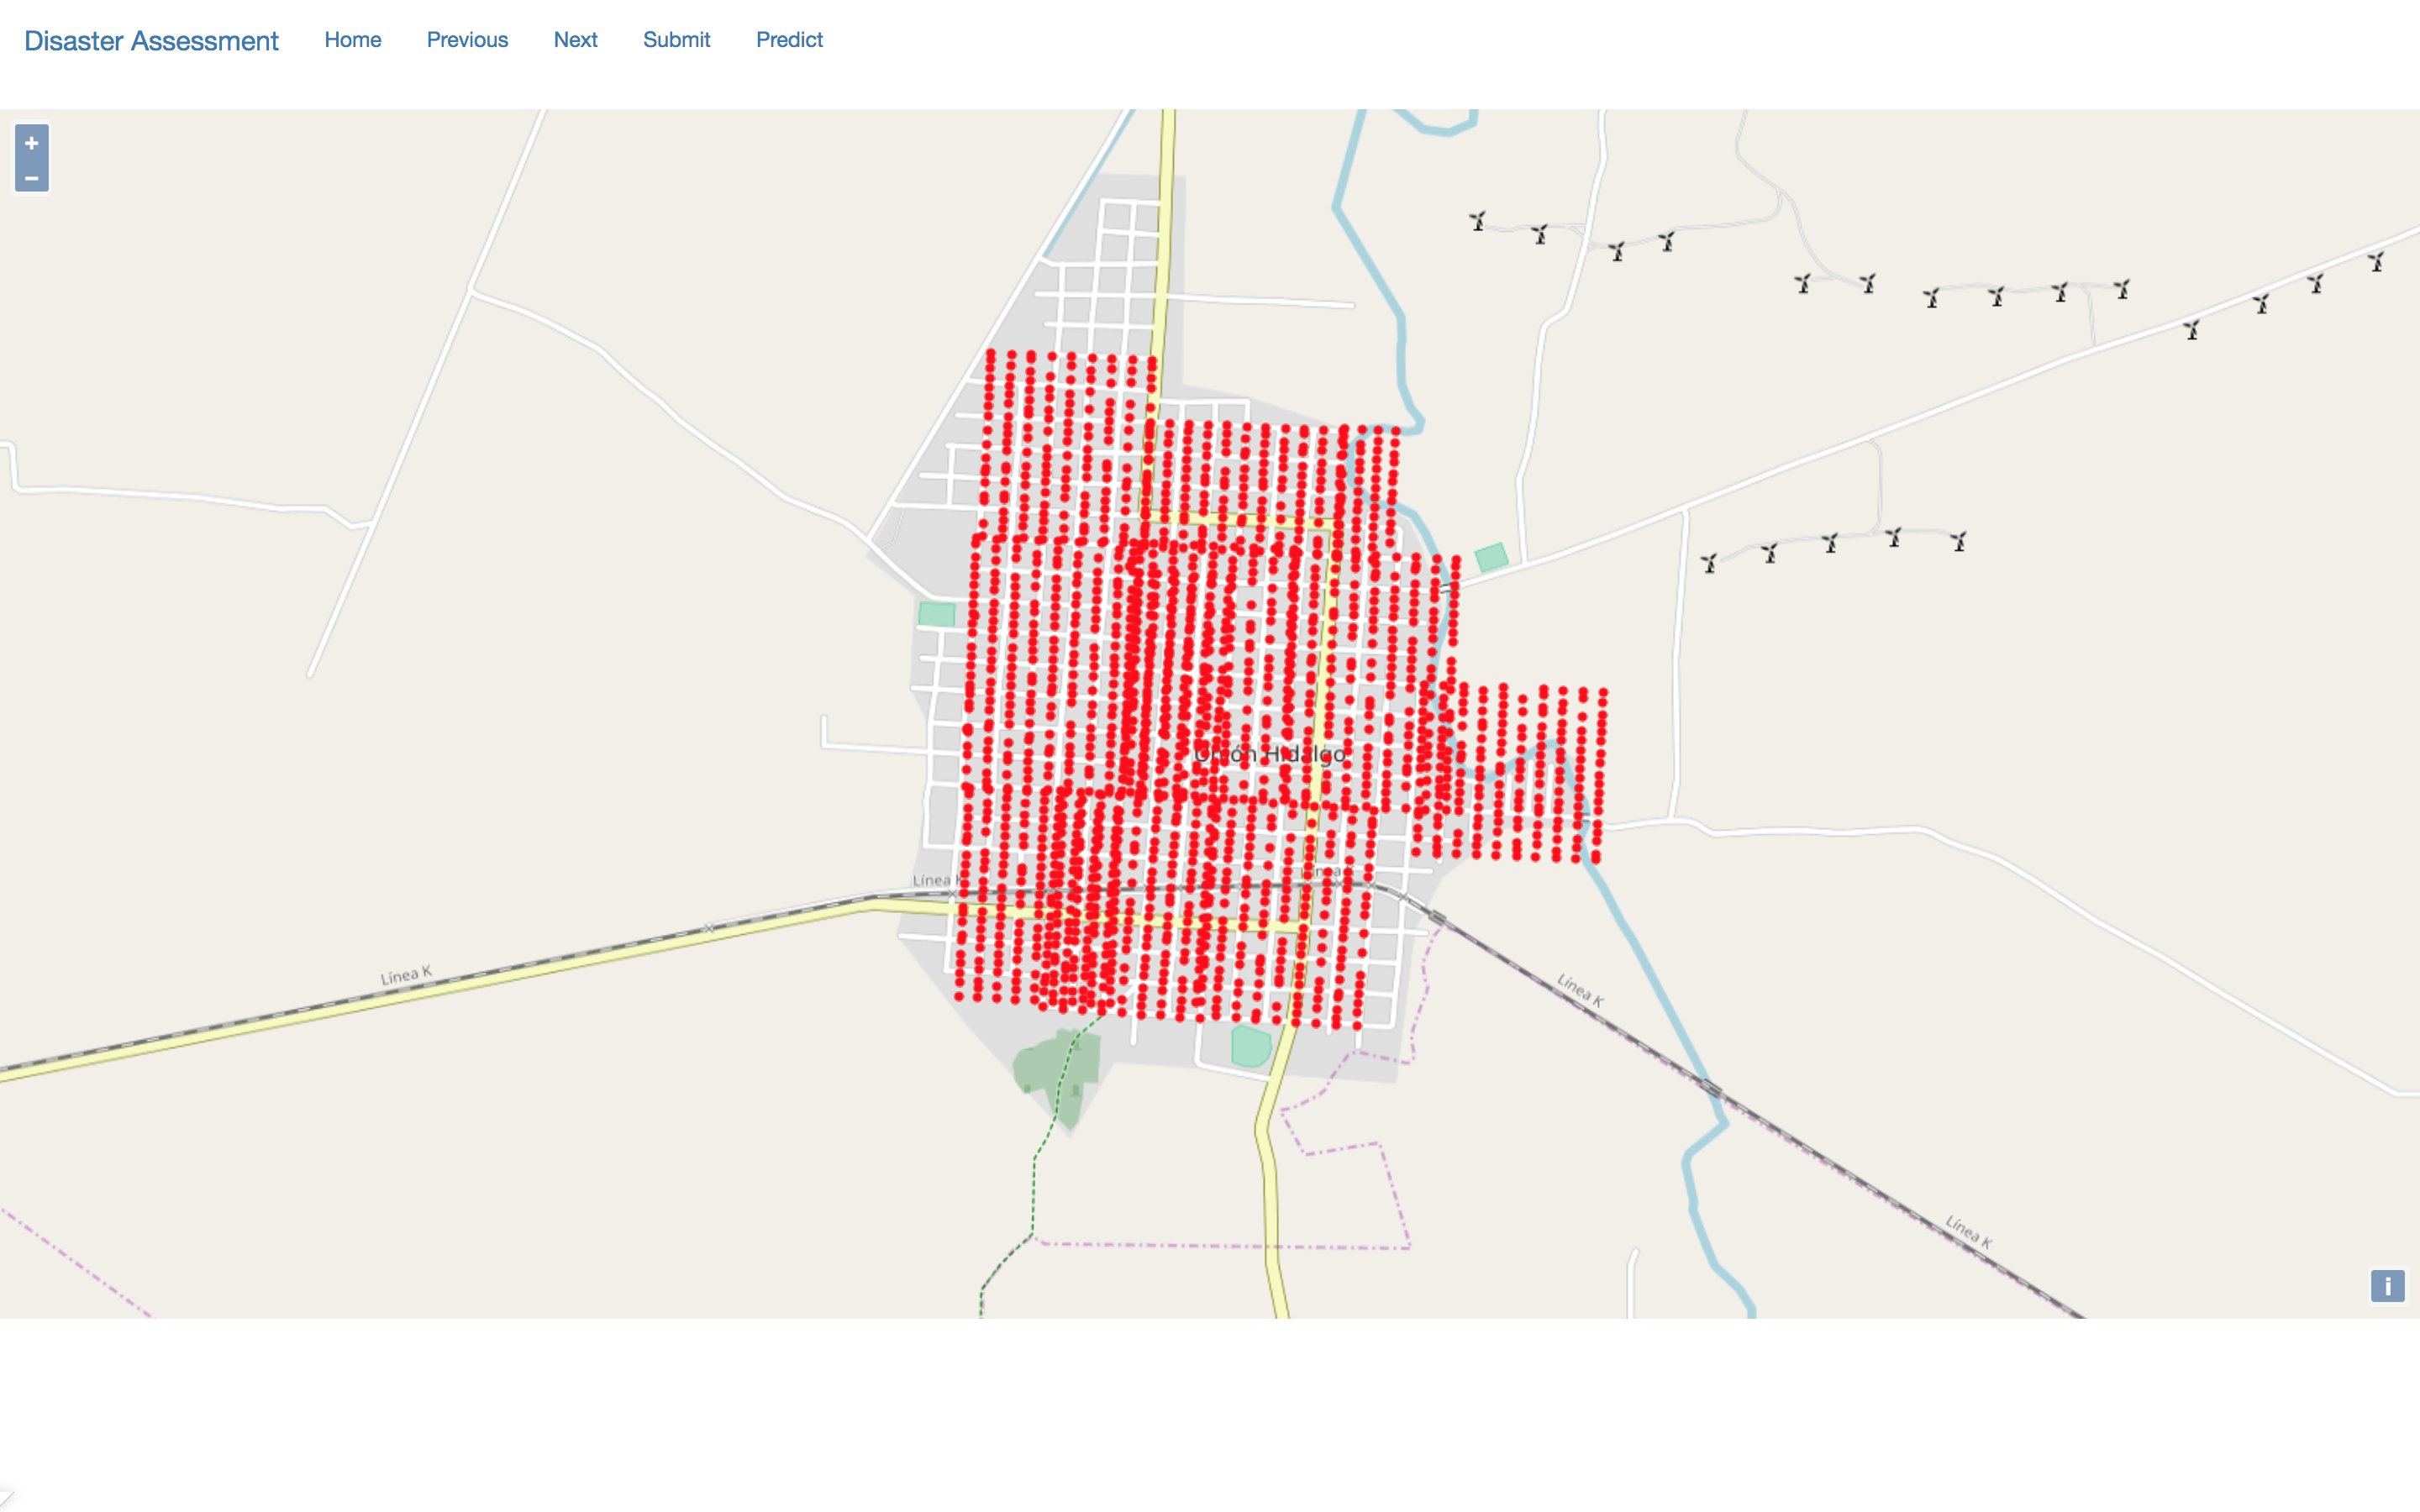
\includegraphics[width=1\textwidth]{images/union.png}}}
  \end{center}
\end{figure}

A t-sne analysis was performed with the images, and it is shown in the figure. To this end, the information from the pixels of each images was flattened into a vector comprising the means and standard deviations. This was a simple dimensionality reduction technique and was useful to embed the images into a lower dimensional space. As we can see, images form natural clusters depending on the town that they where taken from. This was somewhat expected because of the light conditions during the exposure tend to have less variance among similar times and places.


\begin{figure}[h]
  \begin{center}
    \subfigure{\label{fig:tsne}\fbox{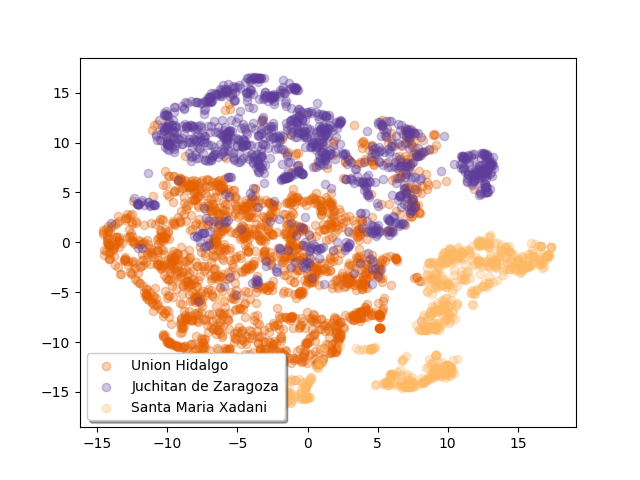
\includegraphics[width=1\textwidth]{images/t-sne.png}}}
  \end{center}
\end{figure}

The results obtained after applying t-sne, supports the proposed methodology of using images from one town, and try to predict on others. Due to the lack of training data, this was needed to be generated from the sample data. The application detailed in the previous chapter was used to crop and classify $100$ square patches from the images in each of the towns. Each patch was $327\times 327$ and a tag was assigined manualy by the author in each of them.

\section{Model validation}

In order to have an effective algorithm we need that it can perform well in places with images it has never seen before. To test this hipothesis we tried two different methodologies based on cross validation. First of all, classic n-fold cross validation was perform on the pool of training data generated for this experiment. This is, the training set was divided in $n$ subsets and then a model was trained using $n-1$ of those sets while the remaining one was used for testing the model. This was repeated n times leaving a different set each time for testing.

\subsection{How much is enough}

In this section we want to create a benchmark on how much images are needed to perform a retraining of the Inception network. What we wanted to achieve was to demonstrate that it is possible to obtain high accuracys using only a handful of images. We where able to test this by designing an experiment that measures the acurracy of models trained with different sizes of training sets and testing them in a common test set. 

\subsection{Computer vision versus convolutional neural networks}

\begin{figure}[h]
  \begin{center}
    \subfigure{\label{fig:tsne}\fbox{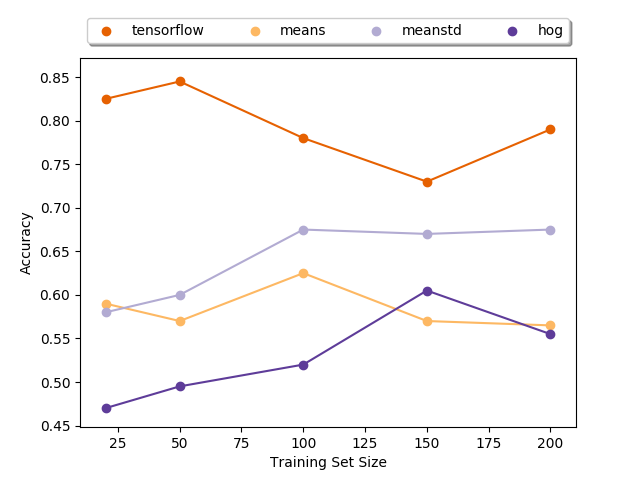
\includegraphics[width=1\textwidth]{images/accuracies-12-3.png}}}
  \end{center}
\end{figure}

\begin{figure}[h]
  \begin{center}
    \subfigure{\label{fig:tsne}\fbox{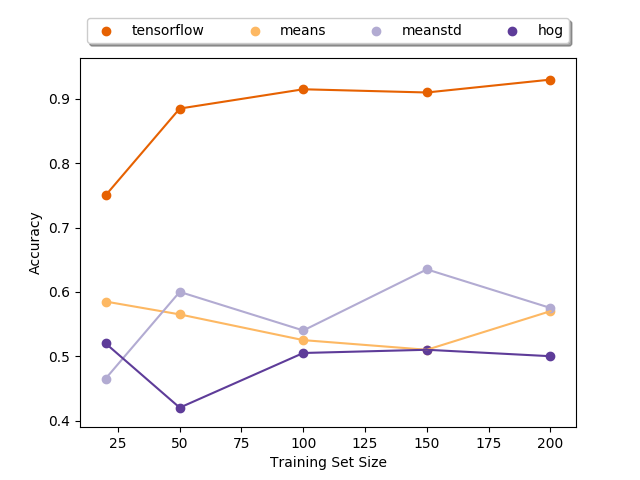
\includegraphics[width=1\textwidth]{images/accuracies-13-2.png}}}
  \end{center}
\end{figure}

\begin{figure}[h]
  \begin{center}
    \subfigure{\label{fig:tsne}\fbox{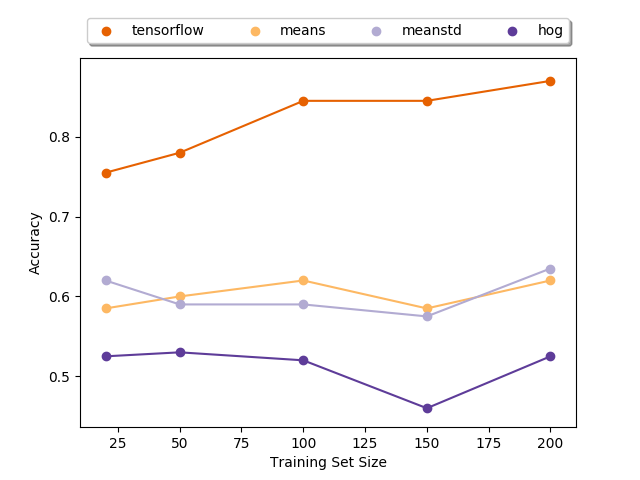
\includegraphics[width=1\textwidth]{images/accuracies-23-1.png}}}
  \end{center}
\end{figure}


\section{Threshold selection}

The binary classifier assigns a real number in the interval $[0,1]$. To decide which values will be assigined with either level a threshold must be chosen. This was picked using a ROC curve. The ROC curve helps us chosing the performance that fits our needs in the ver possible way. In order to do this we use a receiver operating characteristic curve. This tool is often used with binary classifiers to analyse the tradeoff between the true possitive rate and the false possitive rate by selecting different desicion thresholds.

\begin{figure}[h]
  \begin{center}
    \subfigure{\label{fig:tsne}\fbox{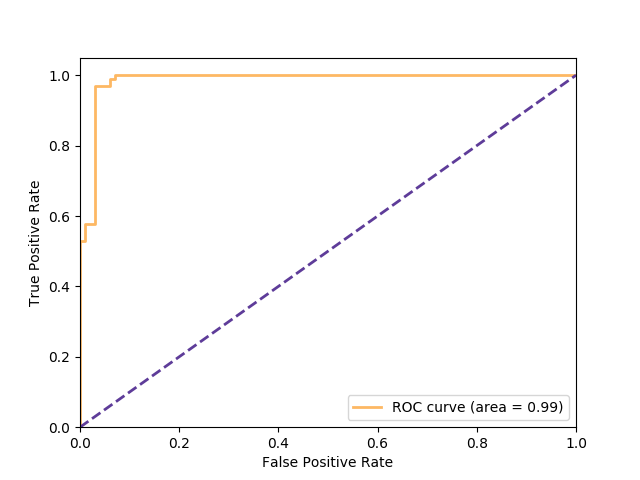
\includegraphics[width=1\textwidth]{images/roc.png}}}
  \end{center}
\end{figure}

The threshold was chosen to keep the false positive rate to 0 percent on the training set while having the highest level of true positive rate. This was atained at the following level:

\begin{center}
  \begin{tabular}{|c|c|c|}
    \hline
    threshold & true positive rate & false positive rate \\ \hline
    0.983629 & 0.529412 & 0.0 \\
    \hline
  \end{tabular}
\end{center}

The reason behind this decision was the high number of false positives shown in preliminary experiments. We want only to look at places in which the model is very confident of finding a damaged building. This theshold can be tunned to match the desired behavior in the requiered application.

\section{Results}

Ortorectified mosaics where built by CENAPRED using the very same images taht we used to train our models. This images come in a different format than the images taken by the drones. Additional to the optical information these tif files contain geographical location and can be used to assing a point in space to each pixel in the image. This means that we can not only locate a damaged building in an image, but to link this information with a geographical location in a given projection.\\

The images where divided in a regular grid of 299 pixel tiles with 90 pixel ovelaps. These overlaps are later postprocessed to eliminate the posibility of counting the same building twice. Each tile is exposed to the model which predicts a class on it using the previously selected threshold. 




